\subsection{基本概念和抽象数据类型}
\begin{frame}\ft{\subsecname}
  \begin{dingyi}[栈]
    栈(Stack)是限定仅在表尾进行插入和删除操作的线性表。
  \end{dingyi}
  \begin{itemize}
  \item[$\diamond$] 允许进行插入、删除操作的一端称为栈顶(top),另一端称为栈底(bottom);\\[0.1in]
  \item[$\diamond$] 不含任何数据元素的栈称为空栈;\\[0.1in]
  \item[$\diamond$] 栈又称后进先出(Last In First out)的线性表,简称LIFO结构。
  \end{itemize}•

\end{frame}

\begin{frame}\ft{\subsecname}
  \begin{itemize}
  \item 栈是一种特殊的线性表,仍具有前驱后继关系。\\[0.1in]
  \item 栈限制了插入和删除的位置,这些操作始终只在栈顶进行。于是栈底是固定的,最先进栈的只能在栈底。
  \end{itemize}
\end{frame}
%

\begin{frame}\ft{\subsecname}
设栈$S=(a_1,a_2,\cd,a_n)$,称$a_1$为栈底元素,$a_n$为栈顶元素。

  \begin{figure}
  \centering
  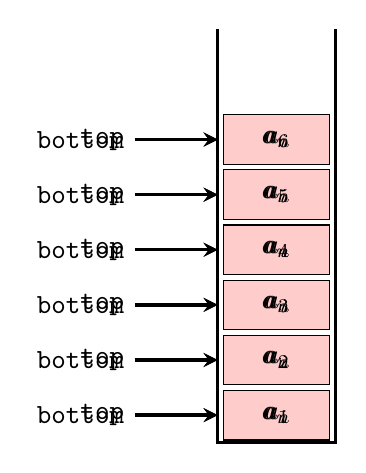
\begin{tikzpicture}
    \tikzstyle{information text}=[rounded corners,fill=blue!20,inner sep=1ex]
    \def\x{1.5}
    \def\y{0.7}
    \def\r{8}
        
    \draw[very thick] (\r,7.5*\y)--(\r,0*\y)--(\r+\x,0*\y)--(\r+\x,7.5*\y);
    
    \foreach \c in {1,2,...,6}{
      \filldraw[fill=red!40,fill opacity=0.5] (\r+0.05*\x,\c*\y-0.95*\y)rectangle(\r+0.95*\x,\c*\y-0.05*\y);
      \ifthenelse{\c=3 \OR \c=5}{
        \node [] at (\r+0.5*\x,\c*\y-0.5*\y) {$\cd$};
      }{
        \ifthenelse{\c=1 \OR \c=2}{
          \node [] at (\r+0.5*\x,\c*\y-0.5*\y) {$a_\c$};
          \ifthenelse{\c=1}{
            \draw[->,>=stealth,very thick] (\r-0.7*\x,\c*\y-0.5*\y) node[left] {\tt{bottom}}--(\r+0,\c*\y-0.5*\y);
          }{}
        }{
          \ifthenelse{4=\c }{
            \node [] at (\r+0.5*\x,\c*\y-0.5*\y) {$a_i$};
          }{
            \node [] at (\r+0.5*\x,\c*\y-0.5*\y) {$a_n$};
            \draw[->,>=stealth,very thick] (\r-0.7*\x,\c*\y-0.5*\y) node[left] {\tt{top}}--(\r+0,\c*\y-0.5*\y);
          }
        }
      }
    }
  \end{tikzpicture}
\end{figure}


\end{frame}
%
%
\begin{frame}\ft{\subsecname}
  \begin{itemize}
  \item 栈的插入操作叫做进栈,也称压栈、入栈。\\[0.1in]
  \item 栈的删除操作叫做出栈,也称弹栈。
  \end{itemize}
\end{frame}

\begin{frame}\ft{\subsecname}

  \begin{figure}
  \centering
  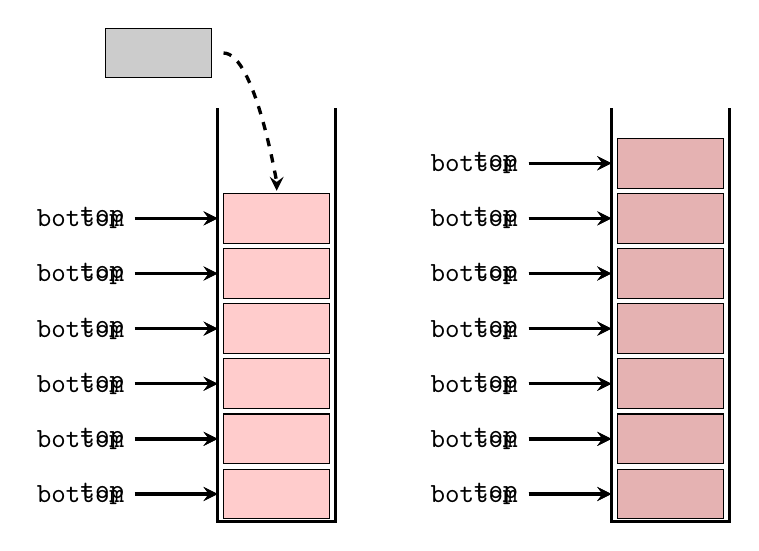
\begin{tikzpicture}
    \tikzstyle{information text}=[rounded corners,fill=blue!20,inner sep=1ex]

    \def\x{1.5}
    \def\y{0.7}
    \def\r{0.5}
    \def\c{9}
    
    \filldraw[fill=black!40,fill opacity=0.5] (\r+0.05*\x,\c*\y-0.95*\y)rectangle(\r+0.95*\x,\c*\y-0.05*\y); 
    \draw[->,>=stealth,dashed,very thick] (\r+1.05*\x,\c*\y-0.5*\y) .. controls +(right:4mm) and +(up:1mm) .. (2+0.5*\x,6*\y);

    \def\r{2}
    \draw[very thick] (\r,7.5*\y)--(\r,0*\y)--(\r+\x,0*\y)--(\r+\x,7.5*\y);
    \foreach \c in {1,2,...,6}{
      \filldraw[fill=red!40,fill opacity=0.5] (\r+0.05*\x,\c*\y-0.95*\y)rectangle(\r+0.95*\x,\c*\y-0.05*\y);
      \ifthenelse{\c=1}{
        \draw[->,>=stealth,very thick] (\r-0.7*\x,\c*\y-0.5*\y) node[left] {\tt{bottom}}--(\r+0,\c*\y-0.5*\y);
      }{}
      \ifthenelse{\c=6}{
        \draw[->,>=stealth,very thick] (\r-0.7*\x,\c*\y-0.5*\y) node[left] {\tt{top}}--(\r+0,\c*\y-0.5*\y);
      }{}
    }

    \pause 
    \def\r{7}
    \draw[very thick] (\r,7.5*\y)--(\r,0*\y)--(\r+\x,0*\y)--(\r+\x,7.5*\y);
    \foreach \c in {1,2,...,7}{
      \ifthenelse{\c=7}{
        \filldraw[fill=black!40,fill opacity=0.5] (\r+0.05*\x,\c*\y-0.95*\y)rectangle(\r+0.95*\x,\c*\y-0.05*\y);
        \draw[->,>=stealth,very thick] (\r-0.7*\x,\c*\y-0.5*\y) node[left] {\tt{top}}--(\r+0,\c*\y-0.5*\y);
      }{
        \filldraw[fill=red!40,fill opacity=0.5] (\r+0.05*\x,\c*\y-0.95*\y)rectangle(\r+0.95*\x,\c*\y-0.05*\y);
      }
      
      \ifthenelse{\c=1}{
        \draw[->,>=stealth,very thick] (\r-0.7*\x,\c*\y-0.5*\y) node[left] {\tt{bottom}}--(\r+0,\c*\y-0.5*\y);
      }{}
      
    }
  \end{tikzpicture}
  \caption{进栈}
\end{figure}


\end{frame}

\begin{frame}\ft{\subsecname}

  \begin{figure}
  \centering
  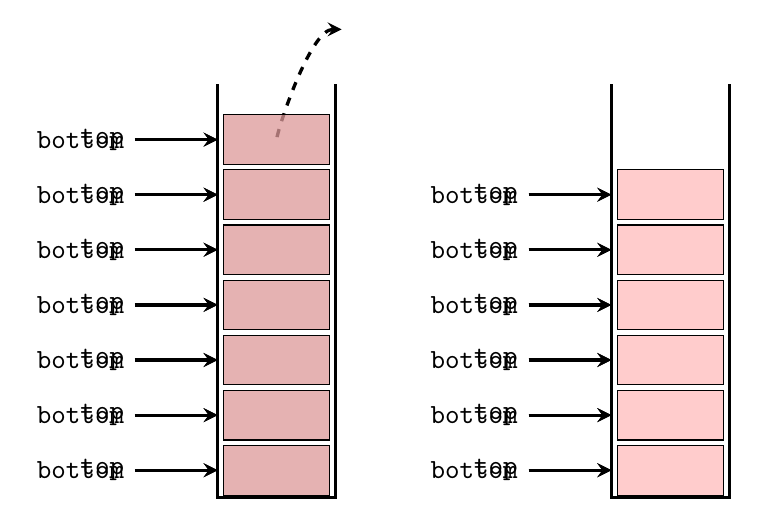
\begin{tikzpicture}
    \tikzstyle{information text}=[rounded corners,fill=blue!20,inner sep=1ex]

    \def\x{1.5}
    \def\y{0.7}
    \def\r{0.5}
    \def\c{9}
    
    \draw[<-,>=stealth,dashed,very thick] (\r+2.05*\x,\c*\y-0.5*\y) .. controls +(left:4mm) and +(up:1mm) .. (2+0.5*\x,6.5*\y);

    \def\r{2}
    \draw[very thick] (\r,7.5*\y)--(\r,0*\y)--(\r+\x,0*\y)--(\r+\x,7.5*\y);
    \foreach \c in {1,2,...,7}{
      \ifthenelse{\c=7}{
        \filldraw[fill=black!40,fill opacity=0.5] (\r+0.05*\x,\c*\y-0.95*\y)rectangle(\r+0.95*\x,\c*\y-0.05*\y);
        \draw[->,>=stealth,very thick] (\r-0.7*\x,\c*\y-0.5*\y) node[left] {\tt{top}}--(\r+0,\c*\y-0.5*\y);
      }{
        \filldraw[fill=red!40,fill opacity=0.5] (\r+0.05*\x,\c*\y-0.95*\y)rectangle(\r+0.95*\x,\c*\y-0.05*\y);
      }
      
      \ifthenelse{\c=1}{
        \draw[->,>=stealth,very thick] (\r-0.7*\x,\c*\y-0.5*\y) node[left] {\tt{bottom}}--(\r+0,\c*\y-0.5*\y);
      }{}
      
    }

    \pause 

    \def\r{7}
    \draw[very thick] (\r,7.5*\y)--(\r,0*\y)--(\r+\x,0*\y)--(\r+\x,7.5*\y);
    \foreach \c in {1,2,...,6}{
      \filldraw[fill=red!40,fill opacity=0.5] (\r+0.05*\x,\c*\y-0.95*\y)rectangle(\r+0.95*\x,\c*\y-0.05*\y);
      \ifthenelse{\c=1}{
        \draw[->,>=stealth,very thick] (\r-0.7*\x,\c*\y-0.5*\y) node[left] {\tt{bottom}}--(\r+0,\c*\y-0.5*\y);
      }{}
      \ifthenelse{\c=6}{
        \draw[->,>=stealth,very thick] (\r-0.7*\x,\c*\y-0.5*\y) node[left] {\tt{top}}--(\r+0,\c*\y-0.5*\y);
      }{}
    }
  \end{tikzpicture}
  \caption{出栈}
\end{figure}


\end{frame}


\begin{frame}[fragile]\ft{\subsecname}   
\begin{lstlisting}[mathescape=true]
    ADT Stack{
      Data:
      `同线性表。元素具有相同的数据类型,相邻元素有前驱、后继关系。`
      Operation:
      Init(*S):     `初始化操作,创建一个空栈S`
      Destroy(*S):  `若栈存在,销毁之`
      Clear(*S):    `将栈清空`
      IsEmpty(S):   `若栈为空,返回true;否则返回false`
      GetTop(S,*e): `若栈存在且非空,用e返回栈顶元素`
      Push(*S,e):   `若栈存在,插入新元素e并称为栈顶元素`
      Pop(*S,*e):   `删除栈顶元素,并用e返回其值`
      Length(S):   `返回元素个数`
    } ADT Stack
  \end{lstlisting}
\end{frame}
